\subsection{Registers} \label{registers}
We are investigating the usefulness of Ampersand for registry systems.
Register systems are also known as registers.
The current \acrshort{big} is housed in a registry system.

The current system developed to support the \acrshort{big} still has the project name Zorro.
This stands for \acrlong{zorro}.
This system was developed in 2008 as a successor to the Ribiz system.
Zorro is a Microsoft.net (C\#) application running on a windows platform with an underlying MS-SQL server.
The architecture of the system is based on an internal workflow, but continuous design changes over the years
has caused a maintenance issue that requires new construction for this system.

The \acrfull{alm} advice~\citepNonPub{de_kok_analyse_2019} has shown that in addition to a maintenance problem, there are also issues in the field of security, outdated architecture and process support.
In consultation with the policy directorate (beleidsdirectie) that is responsible for \acrshort{big}, the CIBG has embarked on a process for new construction.
The \acrshort{alm} advice has been there since 2019.
Preparations for the new building have started, but construction has not yet started.

As mentioned, the current \acrshort{zorro} is built as a workflow system.
The idea behind this was that when adding a new profession within the \acrshort{big} only a new professional title should be added.
Practice proves to be more unruly, and numerous exceptions have been made within the software for trajectories within the professions and specializations.
What does make the software complex is the integration of disciplinary law within \acrshort{zorro}.
Also, the support of the trajectory of foreign persons who want to work in the healthcare field.
This interweaving has made the program great.
The current~\acrfull{sig} rebuild calculation has estimated it at 27 man-years.

\begin{wrapfigure} {r}{0.3\textwidth} 
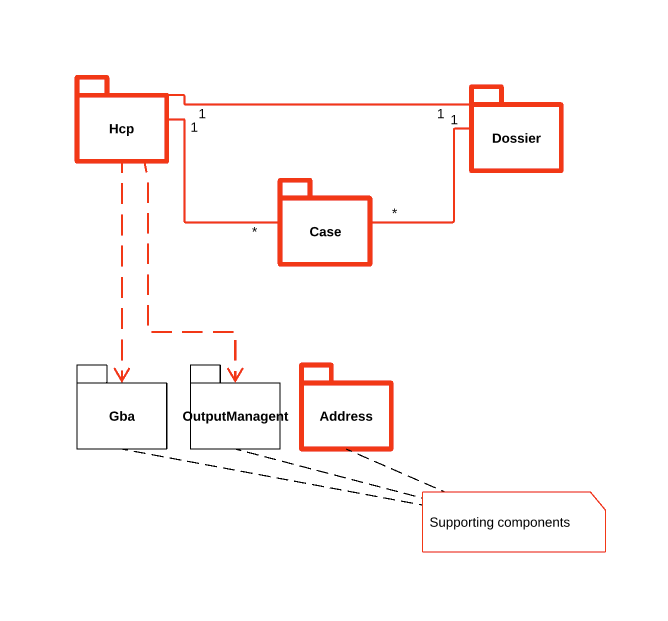
\includegraphics[width=5cm, height=5cm]{overview_zorro.png}
\caption{overview zorro}
\label{fig:overview_zorro}
\end{wrapfigure}
Zorro is divided in several building blocks.
Building blocks related to the persons called~\acrfull{hcp}, concerning the workflow called Case and creating files called Dossier.
The case building block has its focus on the process of registration. 
Looking at the main data model blocks, one can see that it involves metadata, product, state and of course the case and its requests and activities.
On the other hand, the dossier is only about physical documents that are scanned and archived.
Technically, this is solved via a SharePoint solution.
Also, an outdated solution for archiving documents.
The most important building block is about the people who want to be registered.
\begin{figure}
    \centering
    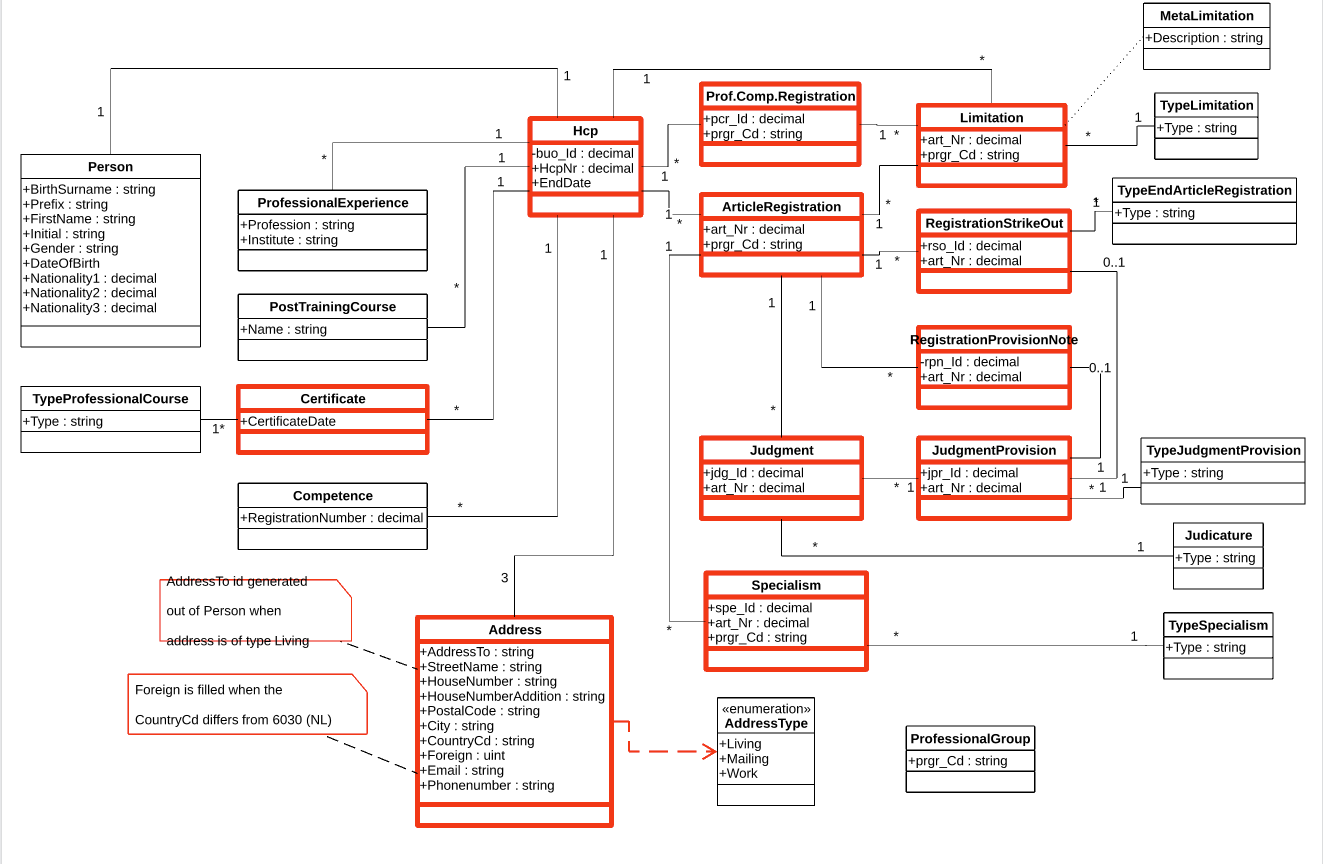
\includegraphics[scale=0.3]{hcp.png}
    \caption{HealthCarePerson}
    \label{fig:hcp}
\end{figure}

During the design, they clearly looked at what the \acrshort{big} has in it.
This is also reflected in the current data model.
One sees in this data model the interdependence with the "tucht" process.
It's called Judgment and JudgmentProvisionNote.
All signs of disciplinary action.
The physical implementation of this data model is much more complex.
This is due to the inclusion of foreigners in the system.
